\documentclass[autodetect-engine,dvipdfmx-if-dvi,ja=standard,everyparhook=compat]{bxjsarticle}

\usepackage{graphicx}        % 図を表示するのに必要
\usepackage{color}           % jpgなどを表示するのに必要
\usepackage{amsmath,amssymb} % 数学記号を出すのに必要
\usepackage{type1cm}         % fontsizeのエラー回避
\usepackage{here}            % 図の強制配置
\usepackage{url}             % URLをいい感じにしてくれる
\usepackage{subfigure}       % 図をまとめて表示
\usepackage{pdfpages}        % PDFの連結
\usepackage{setspace}
\usepackage{cases}
\usepackage{fancyhdr}
\usepackage{wrapfig}% 図の回り込み


% 余白の設定
% \setlength{\textheight}{\paperheight}   % 紙面縦幅を本文領域にする(BOTTOM=-TOP)
% \setlength{\topmargin}{-15.4truemm}     % 上の余白を10mm(=1inch-15.4mm)に
% \addtolength{\topmargin}{-\headheight}  %
% \addtolength{\topmargin}{-\headsep}     % ヘッダの分だけ本文領域を移動させる
% \addtolength{\textheight}{-20truemm}    % 下の余白も10mm
% \setlength{\textwidth}{\paperwidth}     % 紙面横幅を本文領域にする(RIGHT=-LEFT)
% \setlength{\oddsidemargin}{-5.4truemm}  % 奇数ページの左の余白を20mm(=1inch-5.4mm)に
% \setlength{\evensidemargin}{-5.4truemm} % 偶数数ページの左の余白を20mm(=1inch-5.4mm)に
% \addtolength{\textwidth}{-40truemm}     % 右の余白も20mm

% タイトル
\title{タイトル}

% ヘッダとフッタの設定
% \lhead{電気電子情報工学実験}
% \chead{}
% \rhead{20315784 佐藤凌雅}
% \lfoot{}
% \cfoot{\thepage} % ページ数
% \rfoot{}

\parindent = 0pt  % 行頭の字下げをしない
\setstretch{1.0}  % 行間

% キャプションの英語化
\renewcommand{\figurename}{Fig.}
\renewcommand{\tablename}{Table}

% 各章,節などタイトルの大きさを変更
% \titleformat*{\section}{\Huge\bfseries}
% \titleformat*{\subsection}{\Large\bfseries}

% 式の番号を(senction_num.num)のようにする
% \makeatletter
% \@addtoreset{equation}{chapter}
% \def\theequation{\thechapter.\arabic{equation}}
% \makeatother

% 呼び出したページのページ番号を消す
\newcommand{\deletePageNum}{
    \thispagestyle{empty}
    \clearpage
    \addtocounter{page}{-1}
}

% urlのフォントを直す
\renewcommand\UrlFont{\rmfamily}


\begin{document}
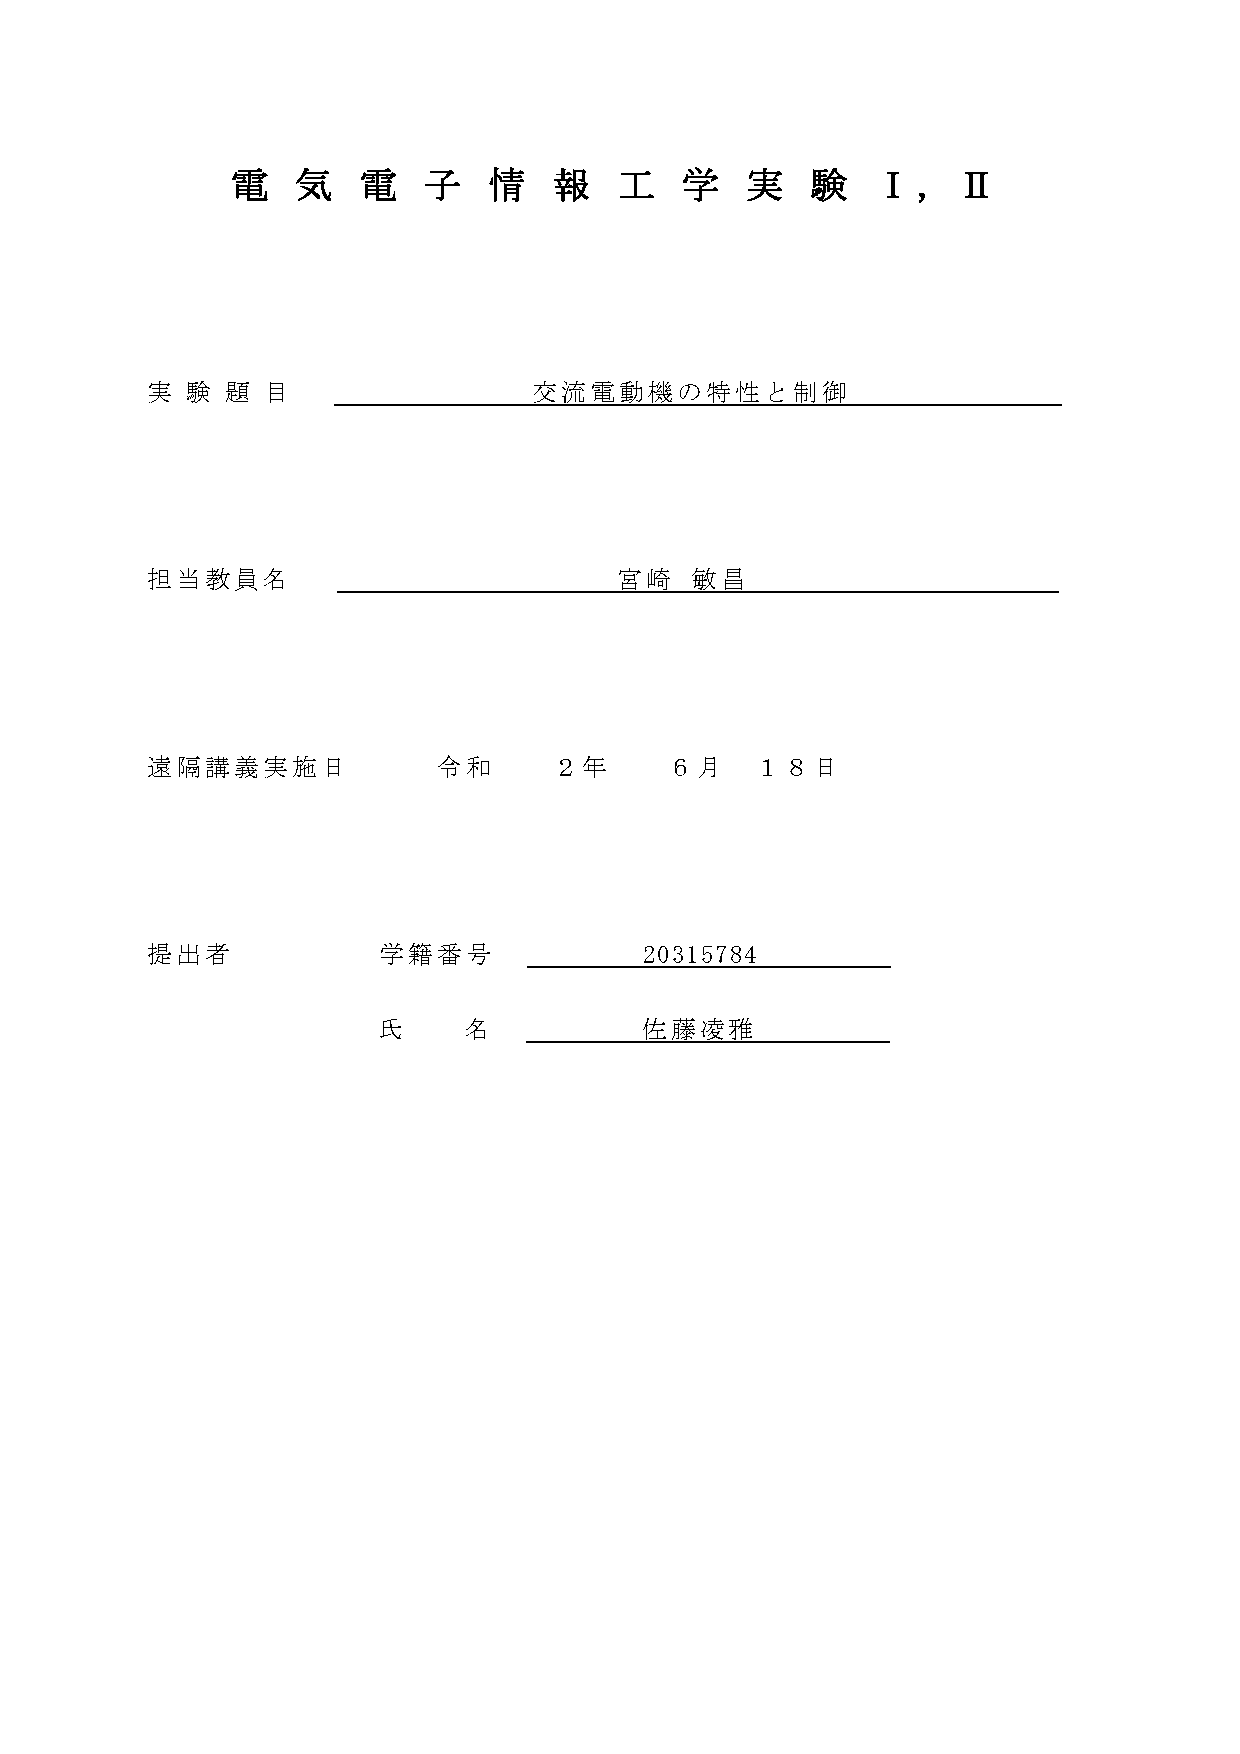
\includepdf[pages=-]{./setting/cover.pdf}
\fontsize{11.041pt}{16.562pt}\selectfont

\section{課題}
\subsection{誘導電動機は身の回りのどこに使われているか?}
 誘導電動機は構造が簡単で丈夫であり,価格が安く,取り扱いが容易であるなどの利点が多いため,工場における大動力用として,また工作機械などの動力用としてよく用いられる.また,身近な例として,電車の動力用モータや,換気扇,洗濯機などの家電の中にも広く使用されている.

\subsection{誘導電動機の電気角速度と機械角速度、すべりの関係について検討せよ.}
 停止している誘導電動機に交流電圧を加えると,回転子導体には大きな誘導電流が流れ,トルクが生じて,回転子が回転する.その回転速度が増して,電気角速度(同期角速度)$\omega$に近づくと,回転子導体の電流は減少し,トルクは小さくなる.機械角速度(回転子の角速度)$\omega_m$は$\omega$より小さく,$\omega$と$\omega_m$の差をすべり角周波数$\omega_s$と呼ぶ.また,$\omega$に対する$\omega_s$の比をすべり$s$という.すなわち,すべり$s$は次の式で表される.
\begin{equation}
    s = \frac{\omega}{\omega_s}
\end{equation}

\subsection{本実験で行う誘導電動機のパラメータ測定法(測定方法とパラメータ導出式)について検討せよ.}
\subsubsection{直流電位降下法}
 測定温度$t$[℃]において,一次巻線の各端子間で測定した抵抗の平均値を$R$[$\Omega$]とし,この値から次の式によって基準巻線温度$T$における一次巻線の1相分の抵抗$r_1$を次の式で計算する.
\begin{equation}
    r_1 = \frac{R}{2} \cdot \frac{235 + T}{235 + t}
\end{equation}

\subsubsection{無負荷試験}
 三相誘導電動機を定格電圧$V_0$[V]で無負荷運転し,その時の無負荷電流$I_0$[A],無負荷入力電力$P_0$[W]を測定する.この測定データから,励磁コンダクタンス$g_0$[S],励磁サセプタンス$b_0$[S]を次の式で計算する.
\begin{eqnarray}
    g_0 &=& \frac{P_0}{V_0^2}\\
    b_0 &=& \sqrt{\left(\dfrac{I_0}{V_0}\right)^2-g_0^2}
\end{eqnarray}

\subsubsection{拘束試験}
 誘導電動機の回転子を回転しないように拘束して,一次巻線に一次電流$I_s$[A]を流した時の一次電圧$V_s$[V],一次入力$P_s$[W]を測定し,励磁回路を除いた等価回路の二次抵抗$r_s$[$\Omega$]および合成リアクタンス$x_s$[$\Omega$]を次の式より計算する.
\begin{eqnarray}
    r_s &=& \frac{P_s}{I_s^2}\\
    x_s &=& \sqrt{\left(\dfrac{V_0}{I_0}\right)^2 - r_s^2}
\end{eqnarray}

\subsection{誘導電動機の一次電流,トルク,機械出力,効率,力率について理論式を検討せよ.}
\subsubsection{一次電流}
 二次電流$I_2$[A]が流れると,$I_2$[A]によって生じる起電力を打ち消すように一次側に一次負荷電流$I_1'$が流れる.ここで,一次巻線と二次巻線の巻数比を$\alpha$とすると,$I_2$[A]と$I_1'$の間には次の関係が成立する.
\begin{equation}
    I_1' = \frac{1}{\alpha} I_2
\end{equation}
 また,一次電流$I_1$[A]は,一次巻線に流れる励磁電流$I_0$[A]と,一時負荷電流$I_1$[A]とのベクトル和になる.
\begin{equation}
    I_1 = I_0 + I_1'
\end{equation}

\subsubsection{トルク}
 電動機のトルクが$T$[N$\cdot$m],角速度が$\omega$[rad/s],回転速度が$n$[min$^{-1}$]とすれば,出力$P_o$[W]は次の式で表現される.
\begin{equation}
    P_o = \omega T = 2 \pi \frac{n}{60} T
\end{equation}
よって,トルク$T$は
\begin{equation}
    T = \frac{60}{2\pi}\cdot\frac{P_o}{n}
\end{equation}

\subsubsection{機械出力}
 1相分の二次入力を$P_2'$[W],二次銅損を$P_{c2}'$[W],機械出力を$P_o'$[W]とすると,次の式が成り立つ
\begin{equation}
    P_2' = I_2^2\frac{r_2}{s} = \frac{P_{c2}'}{s}
\end{equation}
\begin{equation}
    P_o' = P_2'-I_2^2r_2 = P_2'-P_{c2}'=P_2'-sP_2' = (1-s)P_2'
\end{equation}

\subsubsection{効率}
 効率$eta$は機械的出力$P_o$[W],一次銅損$P_{c1}$[W],二次銅損$P_{c1}$[W],鉄損$P_i$[W]を用いて次のように表される.
\begin{equation}
    \eta = \frac{P_o}{P_o + P_{c1} + P_{c2} + P_i}
\end{equation}

\subsubsection{力率}
 力率は次のように表される.
\begin{equation}
    \cos \phi = \frac{\mbox{Re}\left(I_1' + I_0\right)}{\left|I_1' + I_0\right|}
\end{equation}

\subsection{電力変換器を用いた誘導電動機の可変速駆動方式について調査せよ.}
 誘導電動機は本質的には電源の周波数によって決まる同期速度にほぼ近い一定の速度でしか回転しえない.そのため,可変速運転を行うためには工夫が必要である.そこで,入力された交流電流を一度コンバータで直流に変換し,直流電流をインバータを通して再度交流に戻して制御を行う.速度可変は,直流を交流に変換するインバータにて,周波数や電圧を変更することで実現される.

\subsection{次の述語について説明せよ.定格,効率,損失,負荷,トルク,力行および回生.}
\subsubsection{定格}
 誘導電動機を使用する上で,電圧,電流,出力,回転速度などについて,標準的な使い方を示す値.

\subsubsection{効率}
 入力電力に対する機械出力の比のこと.

\subsubsection{損失}
 電動機に入力された電力は鉄損や銅損,機械損などの損失を受けるため,100\%機械的エネルギーに変換されることはない.

\subsubsection{負荷}
 電動機の軸の回転を妨げるように働く力のこと.

\subsubsection{トルク}
 回転体が回転する力のこと.力と回転半径の積で与えられる.

\subsubsection{力行}
 動力車の動力機関が力を動軸に与え,動輪を駆動して走行している状態.

\subsubsection{回生}
 機器で生じる余剰なエネルギーを回収し,電力に変換して再利用すること.例えば,車両において減速の際にタイヤの回転で生じる運動エネルギーを使用して電動機を駆動させて発電を行う.発電された電力を回収することで電力を再利用できるため,エネルギー効率が向上する.


% % 実験の目的,手段,結果,結論を簡潔にまとめ示すこと.(250字程度)
% \section{概要 Abstract}


% % テキストに書かれている目的等を参考に,各自どの点に注目して実験したのかを明確に示すこと.(300字程度)
% \section{目的 Purpose}


% % 各自の実験目的に必要な理論的な背景を示すこと.必要ならば,参考文献リストより文献番号を引用すること.(レポート用紙1枚程度)
% \section{理論的背景 Theory}


% % 実験手段,測定系の概要,測定装置の名称・型番等を書くこと.また,装置の精度・仕様等の情報もできる限り示すこと.(レポート用紙2枚程度)
% \section{実験方法 Experiment}


% % 各自の実験目的に沿った結果を簡潔にまとめること.その他の試行錯誤的実験データは Appendix にまとめる.枚数は各教員の指示に従ってください.(レポート用紙の枚数は教員の指示に従う)
% \section{実験結果 Results}

% % 各自の目的と照らし合わせ,測定結果の妥当性や数値計算結果との整合性などについて考察する.実験結果とサブテキスト/参考書の図式とを比較し議論すること.課題が与えられているテーマに関してはそれについても考察すること.(レポート用紙2枚程度)
% \section{考察 Discussion}

% % 君自身が実験を通じて(実験の方法,まとめ方などで)工夫した点をまとめる.(100字程度 )
% \section{工夫した点}

% 実験結果の羅列ではなく,考察した結果をまとめること.(250字程度)
% \section{まとめ Conclusion}

% レポートで引用した参考文献のリストを付ける.
\begin{thebibliography}{9}
    \bibitem{denkikigairon} 深尾正 (2015). 電気機器概論. 実教出版株式会社.
\end{thebibliography}


% % 周辺の関連調査事項,作成プログラムリスト,試行錯誤的実験データ
% \appendix
% \section{Appendix}

\end{document}
